\newpage
\section{Punto 4}
\textit{Dar ejemplos de los siguientes grafos o explicar por qué tales ejemplos no pueden existir.
\begin{enumerate}
  \item Grafo con un circuito hamiltoniano pero sin un circuito euleriano
  \item Grafo con un circuito euleriano pero sin un circuito hamiltoniano
  \item Grafo con un circuito hamiltoniano y un circuito euleriano
  \item Grafo con un ciclo que incluye todos los vértices pero sin un circuito hamiltoniano ni un circuito euleriano
\end{enumerate}
}

\begin{itemize}
  \item \textbf{Circuito euleriano: }Es un circuito simple que contiene a todas las \underline{aristas} de un grafo G
  \item \textbf{Circuito hamiltoniano: }Es un circuito simple que contiene a todos los \underline{vértices} de un grafo G
\end{itemize}

\begin{figure}[!htb]
  \centering
  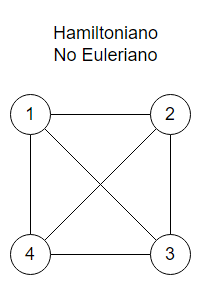
\includegraphics[width=5cm, scale=1]{Images/Punto4/HamiltoniaoNoEuleriano.png}
  \caption{Circuito hamiltoneano no euleriano}
\end{figure}

\begin{figure}
  \centering
  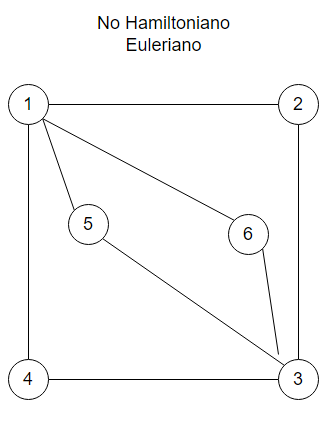
\includegraphics[width=5cm, scale=1]{Images/Punto4/NoHamiltoniaoEuleriano.png}
  \caption{Circuito no hamiltoneano euleriano}
\end{figure}
\begin{figure}
  \centering
  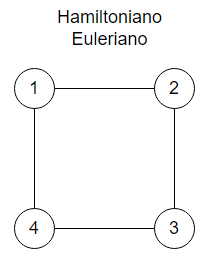
\includegraphics[width=5cm, scale=1]{Images/Punto4/HamiltoniaoEuleriano.png}
  \caption{Circuito hamiltoneano euleriano}
\end{figure}
\begin{figure}
  \centering
  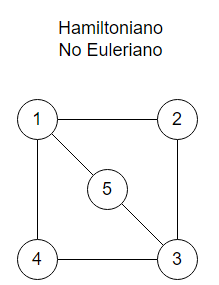
\includegraphics[width=5cm, scale=1]{Images/Punto4/NoHamiltoniaoNoEuleriano.png}
  \caption{Circuito no hamiltoneano no euleriano}
\end{figure}
